\documentclass{article}
\usepackage{hyperref}
\usepackage{amsmath,amssymb}
\usepackage{graphicx}
\usepackage{caption}
\usepackage{subcaption}
\usepackage{color}
\usepackage[section]{placeins}
\renewcommand{\thesubsection}{\thesection.\alph{subsection}}
\usepackage{listings}

\title{Validation and Uncertainty Quantification Proposal for a
Solar-driven Vortex Apparatus} 
\author{Nicholas Malaya\\ Department of Mechanical Engineering \\
University of Texas at Austin}  
\date{}

\begin{document}
\maketitle
\newpage

\section{Introduction}


Renewable energy is critical to our environmental, economic, and
national security. Demand for energy is on the rise, as is our national
reliance on fossil fuel-based power plants for the bulk of our
electricity generation. There is a critical need for safe, clean, and
cost-effective alternatives to coal, such as wind, solar, hydroelectric,
and geothermal power\cite{arpa-e}. These technologies would reduce carbon dioxide
emissions and help position the U.S. as a leader in the global renewable
energy industry. This proposal details a validation plan to build
confidence in a numerical investigation for the design and optimization
of a novel device for renewable, clean energy generation. 

Much of the solar energy incident on the Earth's surface is absorbed
into the ground, which in turn heats the air layer above the surface.
This buoyant air layer contains considerable gravitational potential
energy. The basic idea behind this engineering approach is to convert the 
potential energy in this buoyant air layer to kinetic energy in an
anchored vortex, and to use that kinetic energy to drive a
vertical-axis turbine coupled with an electric generator in order to
produce electrical power. The mechanism is much like that of a naturally
occurring ``dust devil'' with baroclinic generation of vorticity in a
vertically stratified, ground-heated air layer producing a columnar vortex. 

With nearly one-third of global land mass covered by deserts, there are huge
untapped regions for capturing solar heat (about 200 W/$m^2$ averaged over
a 24-hour day, and up to 1000 W/$m^2$ peak).  The available power is
competitive in magnitude with worldwide power generation from fossil
sources. If successful, this could result in a low-cost, scalable
approach to electrical power generation that could create a new class of
renewable energy ideally suited for arid low-wind regions. 

The SoV phenomena has already been demonstrated in an experimental setup
by our partners at Georgia Tech. The simulation effort intends to utilize
Computational Fluid Dynamics (CFD) to simulate this Solar-Driven Vortex
(SoV). These computer simulations are intended to discover the optimal
system configuration for a range of scenarios and system sizes. The
results of these simulations will be used as input for the design of a
pilot site in Mesa, Arizona, and eventually, over a range of
scenarios and system sizes. 

In order for these simulations to be generally useful, they must first
be validated against existing experimental data and high fidelity
simulations. These models will then explore regimes and scales where no
experimental measurements presently exist. Characterizing the
uncertainty of predictions resulting from extrapolation is a critical
component in enabling reliable assessments of field performance of the
SoV, as it will guide the commercialization strategy of the product. 

This report provides a ``validation roadmap'' detailing the process by
which an analysis of the uncertainties inherent to this
problem may be characterized.  It will begin with a discussion of the
physics scenario and the mathematical model, as well as detailing the
reliability of each submodel and the systems inputs. We will then
discuss the validation of these models against existing experimental
data and high fidelity simulations. Finally, we will formulate a Bayesian
analysis for a sub-problem, to serve as a representative example of a
probabilistic analysis applied to this project.  

%
%
%
\section{Problem Definition}

\begin{figure}[h]
 \begin{center}
  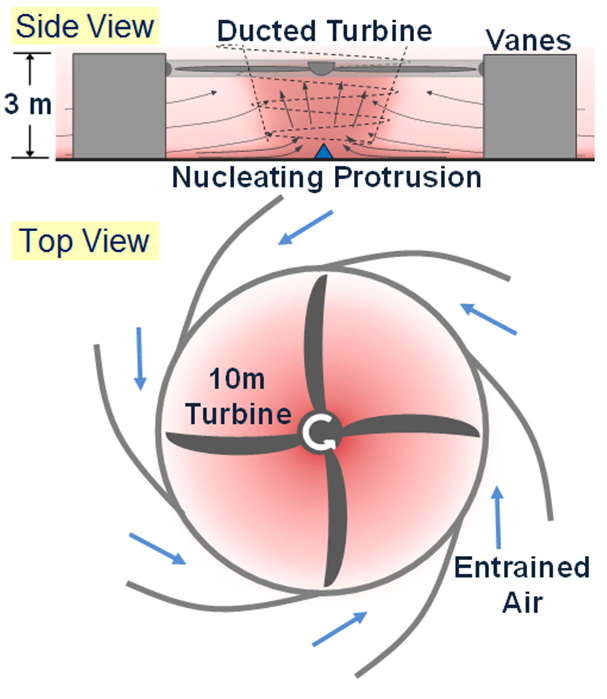
\includegraphics[width=.5\linewidth]{figs/power_generation.png}
   \caption{The Sov facility, showing the vanes, rotor and anchoring
   protrusion, as well as the buoyancy-driven vortex used to drive the
   turbine.}
   \label{facility}
  \end{center}
\end{figure}

The simulations are designed to both mimic the notional SoV experimental
facility as well as identify optimal configurations for future
designs. The general system configuration is depicted in Figure
\ref{facility}. 

Notice several important components of this device. First, ``vanes''
along the sides of the apparatus, designed to entrain outside air and
impart angular momentum. It is not known what configuration and design
of these vanes will lead to optimal dust-devil generation. Thus, these
vanes may have various configurations, varying in the number used, the
length, height, angle of attack. The vanes may also be straight, or
curved.  Next, the ducted turbine above the flow is also a critical design
component. This turbine is designed to extract energy from the flow,
without distrupting/destroying the vortex. Finally, it is desirable to
economically optimize the entire configuration scale by considering both
the power generation, cost of materials, difficulty and expense of
maintainance, etc. 

In addition to the system configuration, it is important to consider the
effect of local conditions on SoV performance. Characterizing the impact
of variations in ambient conditions on the SoV will guide the
commercialization strategy of the product, by determining optimal
install locations across the country. It is therefore desirable to have models
that are capable of accounting for variation in field conditions, such as solar
input, cross-winds and topography. Furthermore, it is expected that 
large ``farms'' of SoVs (akin to the wind and solar farms for wind turbines
and photovoltaics, respectively) may be used by commercial or
utility-scale energy generation. In order for this to be effective, 
the inter-unit spacing must also be optimized, as a single SoV collects
from a large area. These computations will guide commercialization
planning, where decision-makers will need to assess optimum unit size,
spacing, and geographic location for utility-scale deployment.  

%
% 2)
%
\section{Mathematical Specification}



%
% 3)
%
\section{Model Parameter Specification}



%
% 4) Identification of other inputs required for the model (e.g. initial
%   conditions, boundary conditions), and what is known about these
%   inputs for this problem, and associated uncertainties.
%
%
\section{Model Inputs}

The model inputs consistitute a very large component (arguably, the
largest) of the uncertainty in this problem. 

For the Laboratory, 

Initial conditions are highly uncertain. Blowing to cool lab important. 
No sensitivity analysis performed. 

%
% 5) 
%
\section{Proposed Model Calibration}

Lab input conditions


%
% 6)
%
\section{Model Validation}


  \begin{figure}[!htb]
    \begin{center}
     \includegraphics[width = 12 cm]{figs/lab_setup.jpg}
     \caption{The laboratory set-up.}
     \label{lab}
    \end{center}
  \end{figure}

% validation
Several phases of research must be conducted in order to develop robust
and reliable predictive simulation capability. First, the simulations
must be validated against existing experimental data generated from the
laboratory apparatus. These data were taken using particle image
velocimetery (PIV), often not without non-trivial error in measurement and
sampling. In addition, the experimental laboratory has numerous objects
in the immediate vicinity (see figure \ref{lab}) that may
obstruct/manipulate the flow. Finally, as mentioned previously, the
measurements for the cooling, geometry of the room, etc. are rough, and
almost certainly possess non-trivial uncertainties/errors. 



% scaling analysis
New simulations at different conditions will then be performed in order
to inform the optimal design and scale of the planned two and five meter
SoV prototypes, to be installed in Arizona. This study will inform the
design based on the scaling 
of the velocity field and anticipated energy generation. Furthermore,
insights may be gathered on the dyamics of these flows, which could lead
to fundamental advances in the physics of fluid dynamics, dust devils,
and other coherent structures with vortex
dynamics\cite{Mullen1977181,smithleslie,kanak}. Determining the optimal
design of 
these systems will involve parameter sweeps over a large space of
possible configurations. Where possible, models will be developed in
order to simplify the mesh (memory) and computational requirements. One
such method, which replaces the turning vanes with a model, improved
runtime by a factor of twenty-four, due to the greatly decreased
mesh resolution requirements near the vane trailing edges. These models,
once properly validated, will be invaluable tools in effective computer
aided design and simulation of this new technology. 


%
%
%
\section{Further Concerns}

In order for these simulations to be generally useful, they must first
be validated against existing experimental data and high fidelity
simulations. These models will then explore regimes and scales where no
experimental measurements presently exist. Characterizing the
uncertainty of predictions resulting from extrapolation is a critical
component in enabling reliable assessments of field performance of the
SoV, as it will guide the commercialization strategy of the product.

Our focus has therefore moved to a validation study to ensure that the output of the 
numerical simulation agrees with the experimental measurements. In
particular, we have implemented a simulation designed to closely mimic
the 30 degree vane experimental setup. The outputs of the simulation
(velocity field, temperatures, etc. ) are then compared to available
experimental data, which at this time is principally the velocity field
taken by PIV measurements at a variety of time frames near the center of the SoV.  


%
%
%
\section{Probabalistic Formulation on a Sub-Problem}


%
%
%
\section{Conclusions}




%
% end
%
\newpage
This work is supported by the Department of Energy [Advanced Research
Projects Agency-Energy] under Award Number [DE-FOA-0000670].   

\end{document}
